\documentclass[11pt]{article}
\usepackage[letterpaper,tmargin=.75in,lmargin=.75in,rmargin=.75in,bmargin=.75in]{geometry}  
\usepackage{booktabs}
\usepackage{graphicx}
\newcommand{\blist}{
 \begin{list}{$\bullet$}
 { \setlength{\itemsep}{2pt}
     \setlength{\parsep}{0pt}
     \setlength{\topsep}{6pt}
 } }
\newcommand{\elist}{
  \end{list}  }

\def\supsub#1#2{$^{\rm #1}_{#2}$}
\def\sub#1{$_{#1}$}
\def\super#1{\textsuperscript{#1}}
\newcommand{\plex}{$\cdot$}
\newcommand{\unidir}{$\rightarrow$~}
\newcommand{\bidir}{$\leftrightarrow$~}
  
  
  
  
\begin{document}



\subsection*{Strand displacement gate}
The reaction pathway is depicted in Figure~\ref{fig:gate-pathway}. 
Target test tubes are depicted in Figure~\ref{fig:gate-tubes} based on the specification of (Wolfe et al., {\it J Am Chem Soc}, 2017; Supplementary Section S2.2) with the following definitions. 
The total number of target test tubes is $|\Omega| = \sum_{n=1,\dots,N}$ \{Step 0, Step 1\}$_n$  + Crosstalk = $2N + 1$; 
the target test tubes in the multistate test tube ensemble, $\Omega$, are indexed by $h = 1,\dots,2N+1$. $L_{\rm max} = 2$ for 
all tubes.


\paragraph{\bf Reactants for system $n$}
\blist
\item Target: X\sub{n}
\item Gate: \{A\plex B\}\sub{n}
\elist


\paragraph{\bf Elementary step tubes for system $n$}
\blist
\item Step 0\sub{n}: $\Psi^{\rm products}_{0_n} \equiv$ \{X, A\plex B\}\sub{n}; $\Psi^{\rm reactants}_{0_n} \equiv$ \{A, B\}\sub{n};  $\Psi^{\rm exclude}_{0_n}\equiv$ \{X\plex A\}
\item Step 1$_n$: $\Psi^{\rm products}_{1_n} \equiv$ \{X\plex A, B\}$_n$; $\Psi^{\rm reactants}_{1_n} \equiv$ \{X, A\plex B\}$_n$;  $\Psi^{\rm exclude}_{1_n}\equiv \emptyset$  
\elist

\paragraph{\bf Crosstalk tube}
\blist
\item Crosstalk tube: $\Psi^{\rm reactive}_{\rm global} \equiv \cup_{n=1,\dots,N}\{\lambda_n^{\rm reactive}$\};~~$\Psi^{\rm crosstalk}_{\rm global} \equiv \Psi^{L\le L_{\rm max}}_{\rm global} - \cup_{n=1,\dots,N}\{\lambda_n^{\rm cognate}\}$
\elist
The reactive species and cognate products for system $n$ are: 
\blist
\item $\lambda$\supsub{simple}{n}  = \{A\plex B\}\sub{n}
\item $\lambda$\supsub{ss\textrm{-}out}{n}  = \{X, B\}\sub{n}
\item $\lambda$\supsub{ss-in}{n}  = \{A\super{toe}\}\sub{n}
\item $\lambda$\supsub{reactive}{n} = \{A\plex B, X, B, A\super{toe}\}\sub{n}
\item $\lambda$\supsub{cognate}{n} = \{X\plex A, X\plex A\super{toe}\}\sub{n}
\elist
based on the definitions (listed 5$'$ to 3$'$ using the sequence domain notation of Figure~\ref{fig:gate-pathway}):
\blist
\item A $\equiv$ b*-a*
\item A\super{toe} $\equiv$ b*
\item B $\equiv$ a
\item X $\equiv$ a-b
\elist

\clearpage

\begin{figure}
\centering
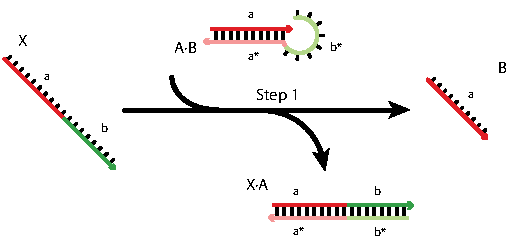
\includegraphics[]{./figs/pathway-displacement}
\bigskip
\bigskip

\begin{footnotesize}
\begin{tabular}{ccp{2.2in}p{2.3in}}
\toprule
Step & Reaction & Function  & Mechanism \\ \midrule
1 & X + A\plex B \unidir  X\plex A + B& detect target X (sequence `a-b') & toehold/toehold nucleation, 3-way branch migration\\
\bottomrule
\end{tabular}
\end{footnotesize}
\bigskip
\caption{Reaction pathway for strand displacement gate. 
A\plex B detects target X (comprising sequence `a-b-c'), generating unstructured output B. Top:~Reaction pathway schematic.  Bottom:~Elementary step details. 
\label{fig:gate-pathway}
    }
\end{figure}



\begin{figure}
\centering
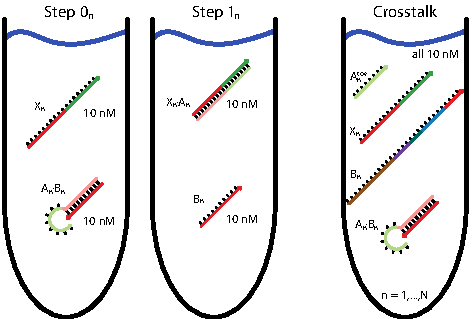
\includegraphics[]{./figs/tubes-displacement}
\bigskip\bigskip
\begin{footnotesize}
\begin{tabular}{lll}
\toprule
Tube & On-targets ($\Psi^{\rm on}_h$)&  Off-targets ($\Psi^{\rm off}_h$) \\ \midrule
Step 0\sub{n} &  \{X, A\plex B\}\sub{n}	& \{A, B\}\sub{n} $\cup~\Psi^{L\le L_{\rm max}}_{0_n}~ -$ \{X\plex A\} \\[3pt]
Step 1\sub{n} &  \{X\plex A, B\}$_n$	& \{X, A\plex B\}\sub{n} $\cup~\Psi^{L\le L_{\rm max}}_{1_n}$ \\[3pt]
Crosstalk & $\cup_{n=1,\dots,N}\{\lambda_n^{\rm reactive}$\} & $\Psi^{L\le L_{\rm max}}_{\rm global} - \cup_{n=1,\dots,N}\{\lambda_n^{\rm cognate}\}$\\
 \bottomrule
\end{tabular}
\end{footnotesize}
\bigskip
\caption{
Target test tubes for strand displacement gate.
Top:~Target test tube schematics. Bottom:~Target test tube details. 
Each target test tube contains the depicted on-target complexes (each with the depicted target structure and a target concentration of 10 nM) 
and the off-target complexes listed in the table (each with vanishing target concentration). To simultaneously design $N$ orthogonal systems, the total number of target test tubes is $|\Omega| = 2N + 1$. $L_{\rm max} = 2$ for all tubes. Design conditions: RNA in 1 M Na$^+$ at 23 $^\circ$C.
        \label{fig:gate-tubes}
    }
\end{figure}
\bigskip



\end{document}